%!TEX root = ../../Bachelorarbeit.tex
\appendixChapter{Quelltexte}
\label{app:anhang}

\section{Quelltext-Beispiel für eine JSON-Transformation und -Validierung}
\lstinputlisting[caption=Beispiel für Play JSON-Transformation bzw. -Validierung, label=app:jsonbsp, language=scala]{code/json_example.scala}

%--------------------------------------------------------------------------------------------------------------------------------------------
\appendixChapter{Interview Protokolle}

\section{Interview 22.11.2012 - Claudia Nikolai }
\label{sec:interview_nikolai}
Claudia Nikolai ist General Programm Manager der D-School.

\subsection*{Zuständigkeiten}
\label{zustaendigkeiten}

\begin{itemize}
\item inhaltliche Programmgestaltung
\item internationale Kooperation
\item Kontakt zu Kunden
\item Ausbildung der Teacher
\item Teacher (an allen Tagen)
\end{itemize}

\subsection*{Austausch mit anderen Teachern}
\label{austauschmitanderenteachern}

\begin{itemize}
\item Teachermeeting
\item E-Mail (Verteiler, Informationen fuer viele Personen)
\item Dropbox\slash E-mail für Content
\end{itemize}

\subsection*{Incom}
\label{incom}

\begin{itemize}
\item space noch nicht privat\slash sichtbar (kein Austausch von vertraulichen Informationen)
\item zu viele Notifications (liest aber alle)
\item nutzt es um Hinweise an andere Teams zu geben
\item sichtet Material an Tagen, an denen keine D-School ist
\end{itemize}

\subsection*{Wichtig für die Dokumentation}
\label{wichtigfuerdiedokumentation}

\begin{itemize}
\item Wie haben die Studenten Empathie bekommen? (Wie und wann haben sie sich in den User hineinvesetzt?)
\item Zitate
\item Dokumentation der Phasen
\item Welche Methode wurde verwendet und wie gut hat sie funktioniert? -> Evaluierung des DS-Prozesses
\end{itemize}

\subsection*{Wunschsystem}
\label{wunschsystem}

\begin{itemize}
\item System sollte einfach verständlich sein, Nutzer haben nur 6--12 Wochen um damit klar zu kommen
\item System muss keine eierlegende Wollmilchsau sein
\end{itemize}

%--------------------------------------------------------------------------------------------------------------------------------------------
\appendixChapter{Ergänzende Visualisierungen}

\section{Datenmodell von Project-Zoom}
In der Abbildung \ref{fig:complete-model} ist das komplette Datenmodell von Project-Zoom dargestellt.
\begin{figure}[h!t]
  \centering     
  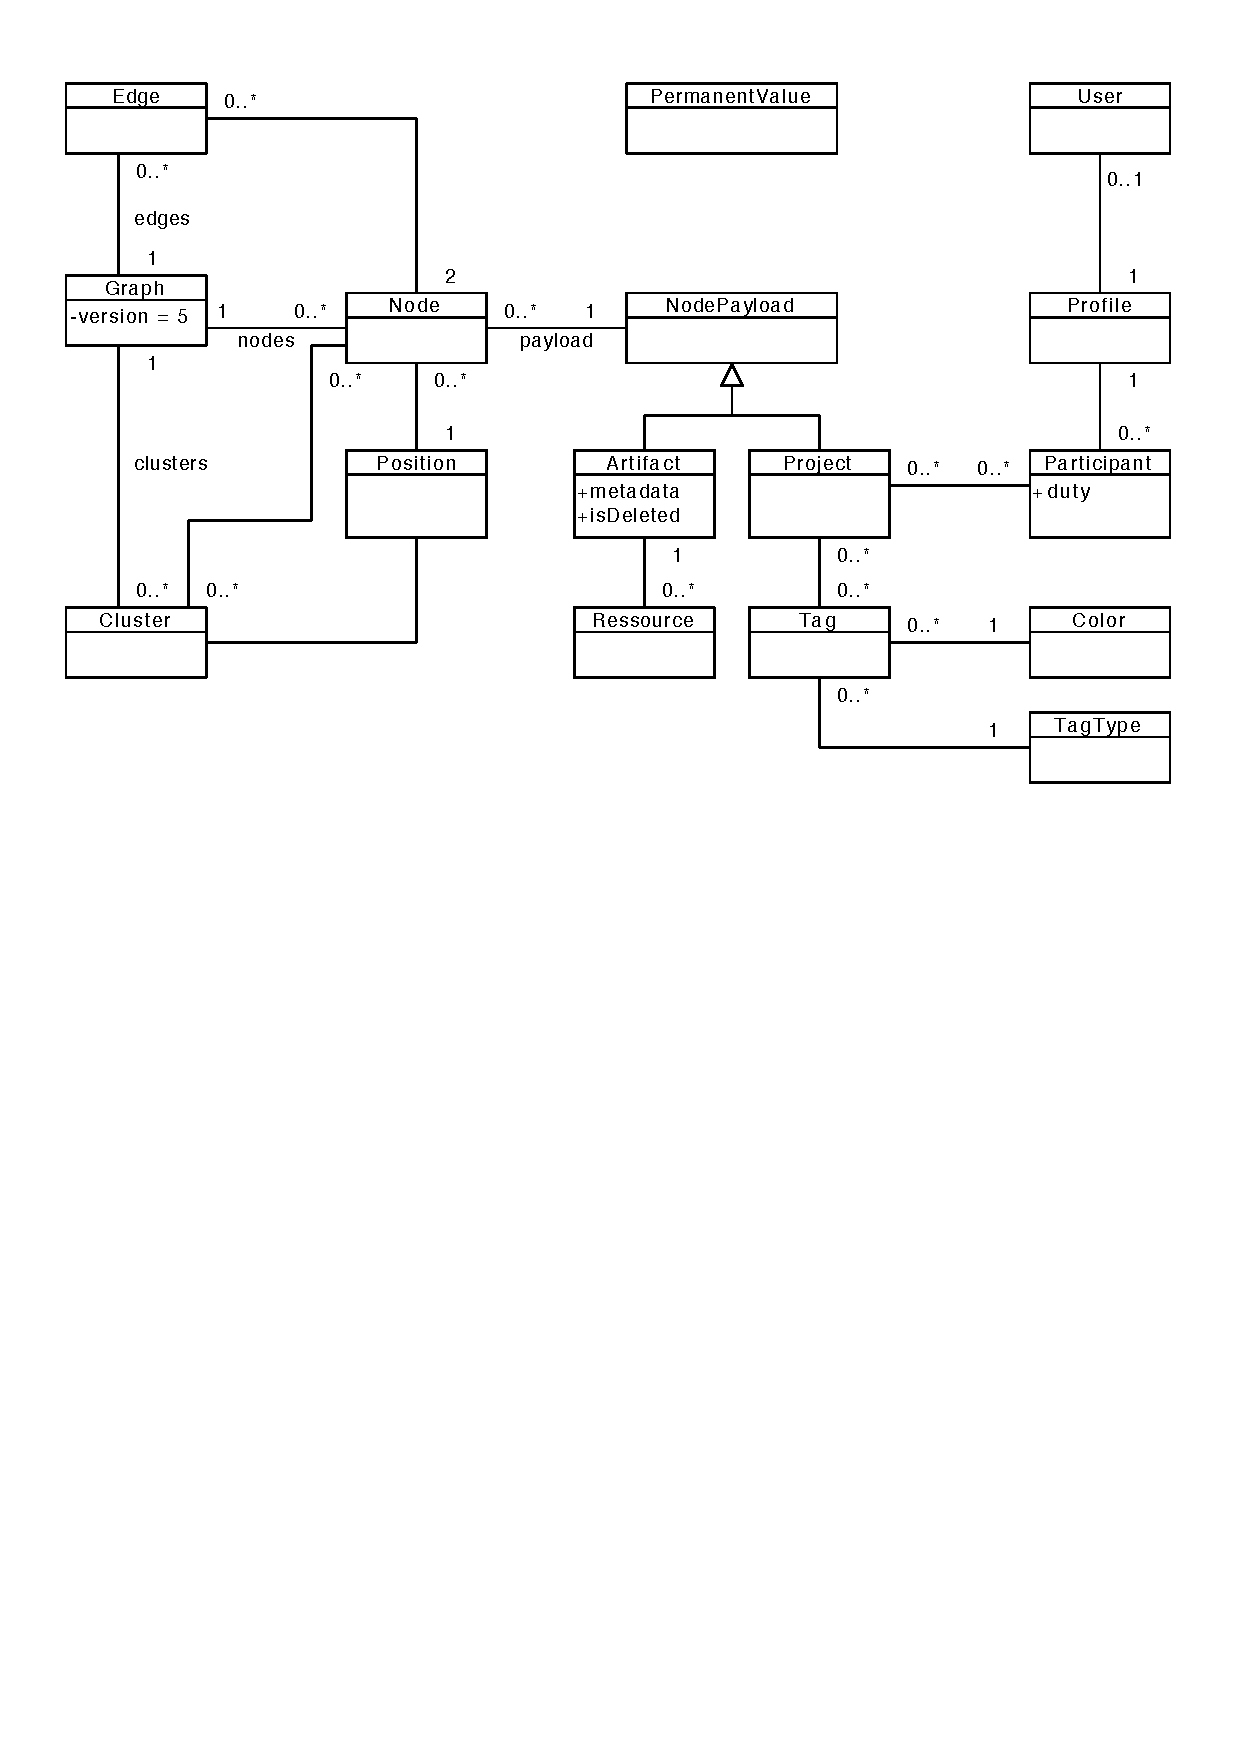
\includegraphics[width=1.0\textwidth]{img/complete_model.pdf}  
   \caption{Datenmodell von Project-Zoom}
  \label{fig:complete-model} 
\end{figure}
\pagebreak
\section{Objektdiagramm für einen beispielhaften Graphen}
\begin{figure}[h!t]
  \centering     
  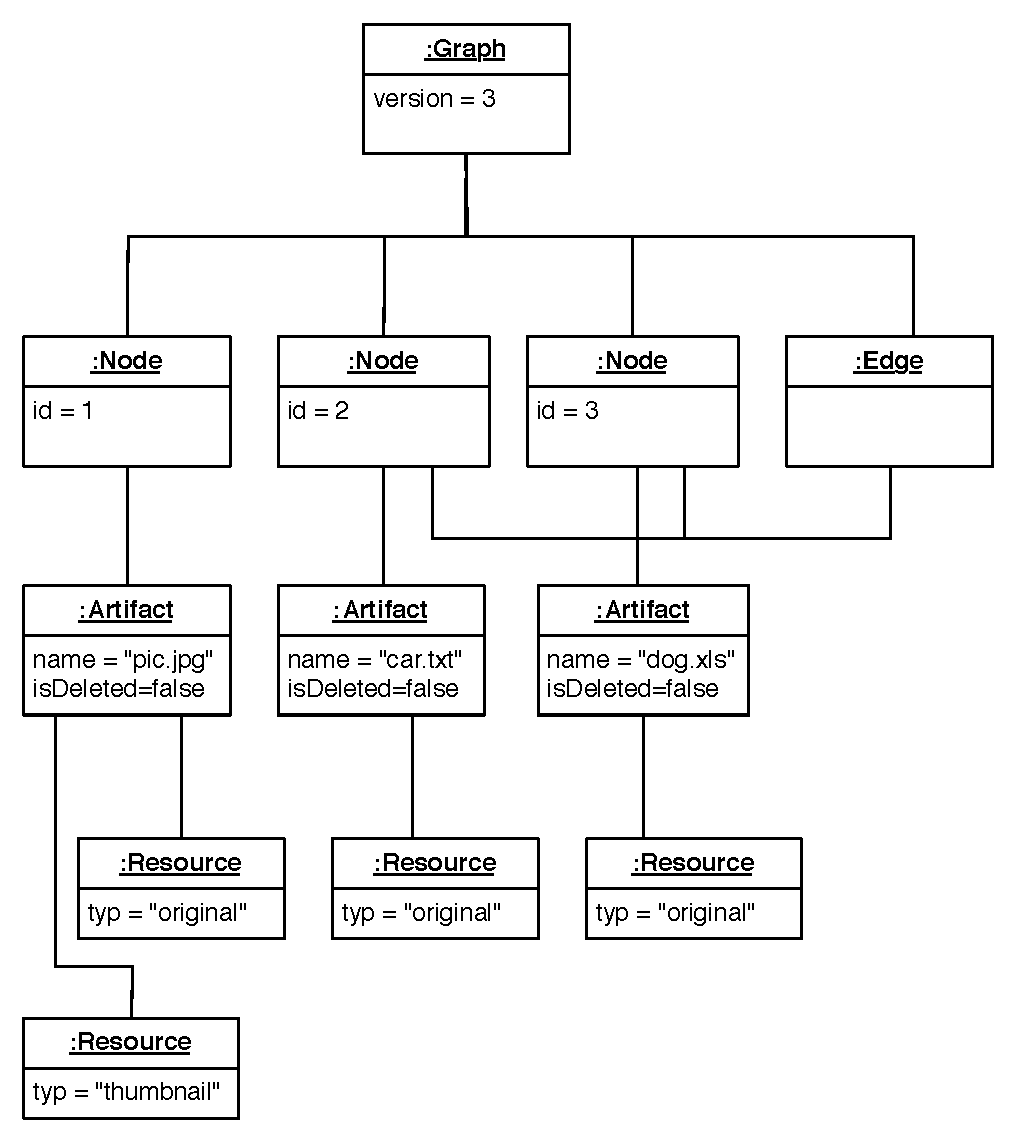
\includegraphics[width=0.8\textwidth]{img/instanz_graph.pdf}  
   \caption{Objektdiagramm eines beispielhaften Graphen. Zur Wahrung der Übersichtlichkeit ist die Position jedes Nodes nicht als Objekt visualisiert.}
  \label{fig:graph-bsp} 
\end{figure}
 
\section{InfoQ Umfrage zu Webframeworks der JVM}
In der Tabelle in der Abbildung \ref{fig:infoq-survey} sind die Umfrageergebnisse der InfoQ-Umfrage mit 1894 Teilnehmern von der Seite \url{http://www.infoq.com/research/jvm-web-frameworks.auf} zum angegebenen Zeitpunkt zu sehen.
\begin{figure}[ht]  
  \centering     
  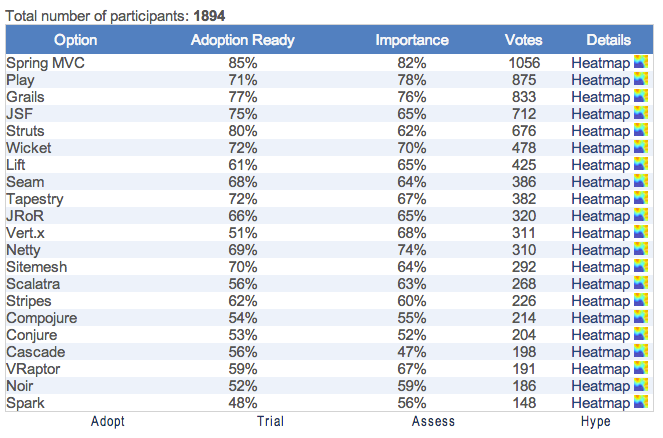
\includegraphics[width=1.0\textwidth]{img/infoq.png}  
   \caption{Stand der Umfrage am 26. Juni 2013}
  \label{fig:infoq-survey} 
\end{figure}

\section{Performance Test}
\label{sec:performance-test}
Project-Zoom wurde mit den folgenden Einstellungen für Apache Bench getestet:
\begin{lstlisting}
ab -g output100.txt -c 10 -n 100000 http://localhost:9000/projects
\end{lstlisting}

Weiterhin wurde noch ein Session-Cookie übergeben, um auf die geschütze Ressource zugreifen zu dürfen. Die Ergebnisse sind in den Abbildungen \ref{fig:perf1} und \ref{fig:perf2} zu sehen. Die Grafiken wurden mit Hilfe von \url{https://loadosophia.org} erstellt.

\begin{figure}
  \centering     
  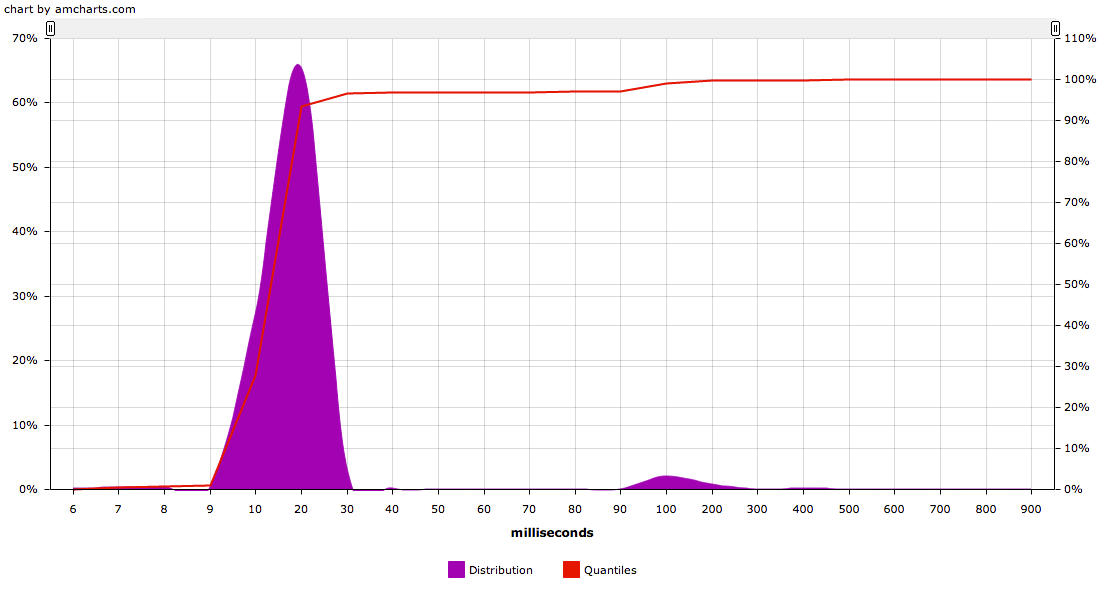
\includegraphics[width=1.0\textwidth]{img/perf1.png}  
   \caption{Dichte- und Verteilungsfunktion der Antwortzeiten }
  \label{fig:perf1} 
\end{figure}

\begin{figure}  
  \centering     
  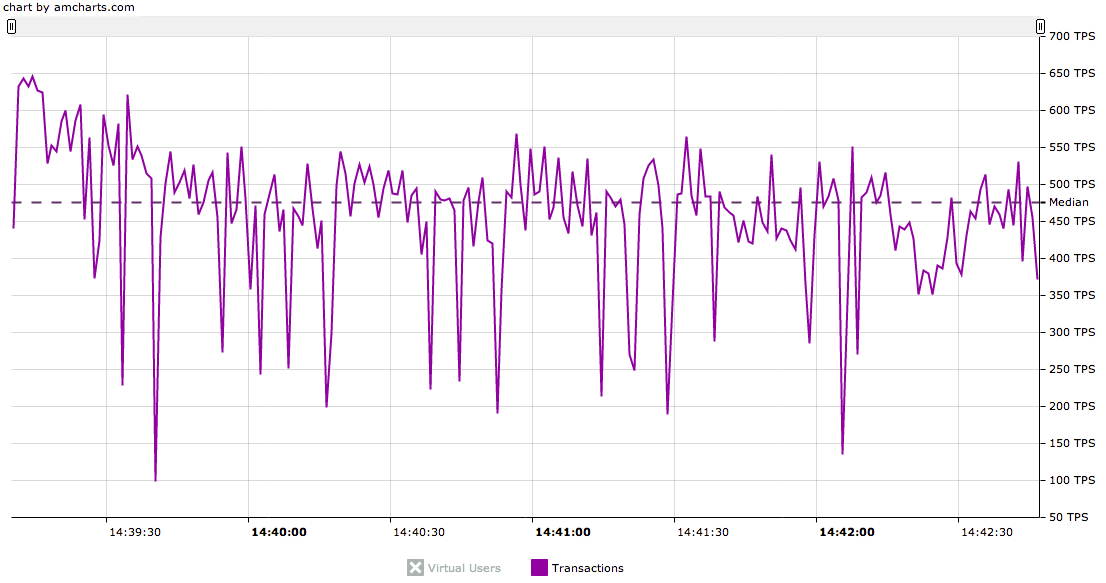
\includegraphics[width=1.0\textwidth]{img/perf2.png}  
   \caption{Durchsatz in abgeschlossenen Übertragungen pro Sekunde über die Zeit}
  \label{fig:perf2} 
\end{figure}


\section{Überblick über die vorhandenen Events}
\label{event-overiview}
In der Tabelle \ref{tab:events} sind alle Events zu sehen, die mit dem Backend-Core interagieren.

\begin{table}
    \begin{tabular}{|l|l|p{4.8cm}|}
    \hline
    ~                   & Parameter                                                                & Bedeutung                                                  \\ \hline
    ArtifactFound       & \begin{lstlisting}[gobble=4] 
    originalStream: InputStream
    artifact: ArtifactLike
    \end{lstlisting}                      & Artefakt von Konnektor gefunden                            \\ \hline
    ArtifactDeleted     & \begin{lstlisting}[gobble=4]
    artifact: ArtifactLike
    \end{lstlisting}                                                   & Löschung von Artefakt durch Konnektor festgestellt         \\ \hline
    ArtifactAggregation & \begin{lstlisting}[gobble=4]
    _project: String
    l: List[ArtifactFound]
    \end{lstlisting}                                 & Auflistung aller Artefakte eines Projektes durch Konnektor \\ \hline
    ArtifactRenamed     & \begin{lstlisting}[gobble=4]
    artifact: ArtifactLike
    name: String
    \end{lstlisting}                                     & Umbenennung von Artefakt durch Konnektor festgestellt      \\ \hline
    ArtifactMoved       & \begin{lstlisting}[gobble=4]
    artifact: ArtifactLike
    path: String
    \end{lstlisting}                                     & Verschiebung von Artefakt durch Konnektor festgestellt     \\ \hline
    ResourceFound       & \begin{lstlisting}[gobble=4]
    inputStream: InputStream
    artifact: ArtifactLike
    resource: ResourceLike
    \end{lstlisting} & Neue Resource für Artefakt gefunden                        \\ \hline
    ArtifactUpdated     & \begin{lstlisting}[gobble=4]
    artifact: ArtifactLike
    \end{lstlisting}                                                   & Artefakt in der DB geändert                                \\ \hline
    ArtifactInserted    & \begin{lstlisting}[gobble=4]
    artifact: ArtifactLike    
    \end{lstlisting}                                               & Artefakt zur DB hinzugefügt                                \\ \hline
    ResourceUpdated     & \begin{lstlisting}[gobble=4]
    file: File
    artifact: ArtifactLike
    resource: ResourceLike
    \end{lstlisting}               & Resource in der DB geändert                                \\ \hline
    ResourceInserted    & \begin{lstlisting}[gobble=4]
    file: File
    artifact: ArtifactLike
    resource: ResourceLike
    \end{lstlisting}               & Resource zur DB hinzugefügt                                \\ \hline
    ProjectFound        & \begin{lstlisting}[gobble=4]
    project: ProjectLike
    \end{lstlisting}                                                     & Projekt von Konnektor gefunden                             \\ \hline
    ProjectAggregation  & \begin{lstlisting}[gobble=4]
    l: List[ProjectFound]      
    \end{lstlisting}                                               & Auflistung mehrerer gefundener Projekte                    \\ \hline
    ProfileFound        & \begin{lstlisting}[gobble=4]
    profile: Profile   
    \end{lstlisting}                                                       & Profil von Konnektor gefunden                              \\ \hline
    ProfileAggregation  & \begin{lstlisting}[gobble=4]
    l: List[ProfileFound]  
    \end{lstlisting}                                                   & Auflistung mehrerer gefundener Profile                     \\ \hline
    GraphUpdated        & \begin{lstlisting}[gobble=4]
    graph: Graph
    patch: JsValue
    \end{lstlisting}                                             & Graph in der DB mit Patch geändert                         \\ \hline
    \end{tabular}
    \caption{Übersicht über Events des Backend-Core}
    \label{tab:events}
\end{table}

\textsc{ArtifactActor}
\begin{labeling}{\textbf{Subscription f{\"u}r:}}
  \item[Publishes] ArtifactUpdated, ArtifactInserted, ResourceUpdated, ResourceInserted
  \item[Subscription f{\"u}r] ArtifactFound, ArtifactDeleted, ArtifactAggregation, ArtifactRenamed, ArtifactMoved, ResourceFound
\end{labeling}

\textsc{KnowledgeActor}
\begin{labeling}{\textbf{Subscription f{\"u}r:}}
  \item[Subscription f{\"u}r] ProjectFound, ProjectAggregation, ProfileFound, ProfileAggregation
\end{labeling}

\textsc{Konnektoren}
\begin{labeling}{\textbf{Subscription f{\"u}r:}}
  \item[Publishes] ProfileAggregation, ProjectAggregation, ArtifactFound, ArtifactRenamed, ArtifactMoved, ArtifactDeleted, ArtifactAggregation
\end{labeling}

\textsc{Thumbnailgenerator}
\begin{labeling}{\textbf{Subscription f{\"u}r:}}
  \item[Publishes] ResourceFound
  \item[Subscription f{\"u}r] ResourceInserted, ResourceUpdated
\end{labeling}

\appendixChapter{REST-Schnittstelle}